\documentclass[11pt]{article}

% Packages
\usepackage{csvsimple}
\usepackage{graphicx}
\usepackage[export]{adjustbox}
\usepackage{caption}
\usepackage{float}
\usepackage{titlesec}
\usepackage{geometry}
\usepackage[hidelinks]{hyperref}
\usepackage{titling}
\usepackage{parskip}
\usepackage{wasysym}
\usepackage{tikzsymbols}
\usepackage{fancyvrb}
\usepackage{xurl}
\usepackage{hyperref}
\usepackage{subcaption}
\usepackage{listings}
\usepackage{xcolor}
\usepackage[spanish]{babel}

% Layout configuration
\geometry{
  left=2.5cm,
  right=2.5cm,
  top=3cm,
  bottom=3cm,
}

\titlespacing{\section}{0pt}{2\parskip}{\parskip}
\titlespacing{\subsection}{0pt}{\parskip}{\parskip}

% Code style configuration
\definecolor{codegreen}{rgb}{0,0.6,0}
\definecolor{codegray}{rgb}{0.5,0.5,0.5}
\definecolor{codepurple}{rgb}{0.58,0,0.82}
\definecolor{backcolour}{rgb}{0.95,0.95,0.92}

\lstdefinestyle{mystyle}{
    backgroundcolor=\color{backcolour},   
    commentstyle=\color{codegreen},
    keywordstyle=\color{magenta},
    numberstyle=\tiny\color{codegray},
    stringstyle=\color{codepurple},
    basicstyle=\ttfamily\footnotesize,
    breakatwhitespace=false,         
    breaklines=true,                 
    numbers=left,                    
    numbersep=5pt,                  
    showspaces=false,                
    showstringspaces=false,
    showtabs=false,                  
    tabsize=2
}

\lstset{style=mystyle}

\begin{document}

\title{Análisis Comparativo de Estrategias de Multiplicación de Matrices con Aceleración GPU}
\author{Adrian Grassin Luis}
\date{\today}
\maketitle

\begin{abstract}
Este estudio analiza y compara tres estrategias diferentes para la multiplicación de matrices: multiplicación por filas, por columnas, y mediante aceleración GPU utilizando OpenCL. Se evalúa el rendimiento de los métodos utilizando matrices de diversos tamaños, con especial énfasis en matrices de gran dimensión, y se analiza el impacto de la arquitectura de memoria y el procesamiento paralelo en el rendimiento.
\end{abstract}

\section{Introducción}
La multiplicación de matrices es una operación fundamental en numerosas aplicaciones computacionales. Este trabajo examina tres implementaciones diferentes de multiplicación de matrices, incluyendo una implementación GPU que aprovecha el hardware de procesamiento paralelo moderno.

\section{Metodología}
\subsection{Entorno de Pruebas}
\begin{itemize}
    \item \textbf{CPU:} AMD Ryzen 5600X
    \item \textbf{GPU:} AMD Radeon RX 7800 XT
    \item \textbf{Lenguaje:} C\# (.NET 8.0)
    \item \textbf{Framework GPU:} OpenCL.NET 2.2.9
    \item \textbf{Patrón de Diseño:} Estrategia (Strategy Pattern)
\end{itemize}

\subsection{Implementaciones}
\begin{itemize}
    \item \textbf{CPU - Por Filas:} Implementación optimizada con procesamiento en bloques y paralelización
    \item \textbf{CPU - Por Columnas:} Implementación optimizada con procesamiento en bloques y paralelización
    \item \textbf{GPU - OpenCL:} Implementación que aprovecha el procesamiento masivamente paralelo de la GPU
\end{itemize}

\subsection{Configuración Experimental}
\begin{itemize}
    \item Tamaños de matriz evaluados: 100x100 hasta 2500x2500
    \item 5 iteraciones por cada tamaño para obtener medias representativas
    \item Elementos de matrices generados aleatoriamente
    \item Medición de tiempos incluyendo transferencia de datos CPU-GPU
\end{itemize}

\section{Resultados y Análisis}
\subsection{Rendimiento Comparativo}
\begin{table}[h]
    \centering
    \csvautotabular{../../results_comparison.csv}
    \caption{Tiempos de ejecución promedio (ms) para diferentes tamaños de matriz}
\end{table}

\begin{figure}[h]
    \centering
    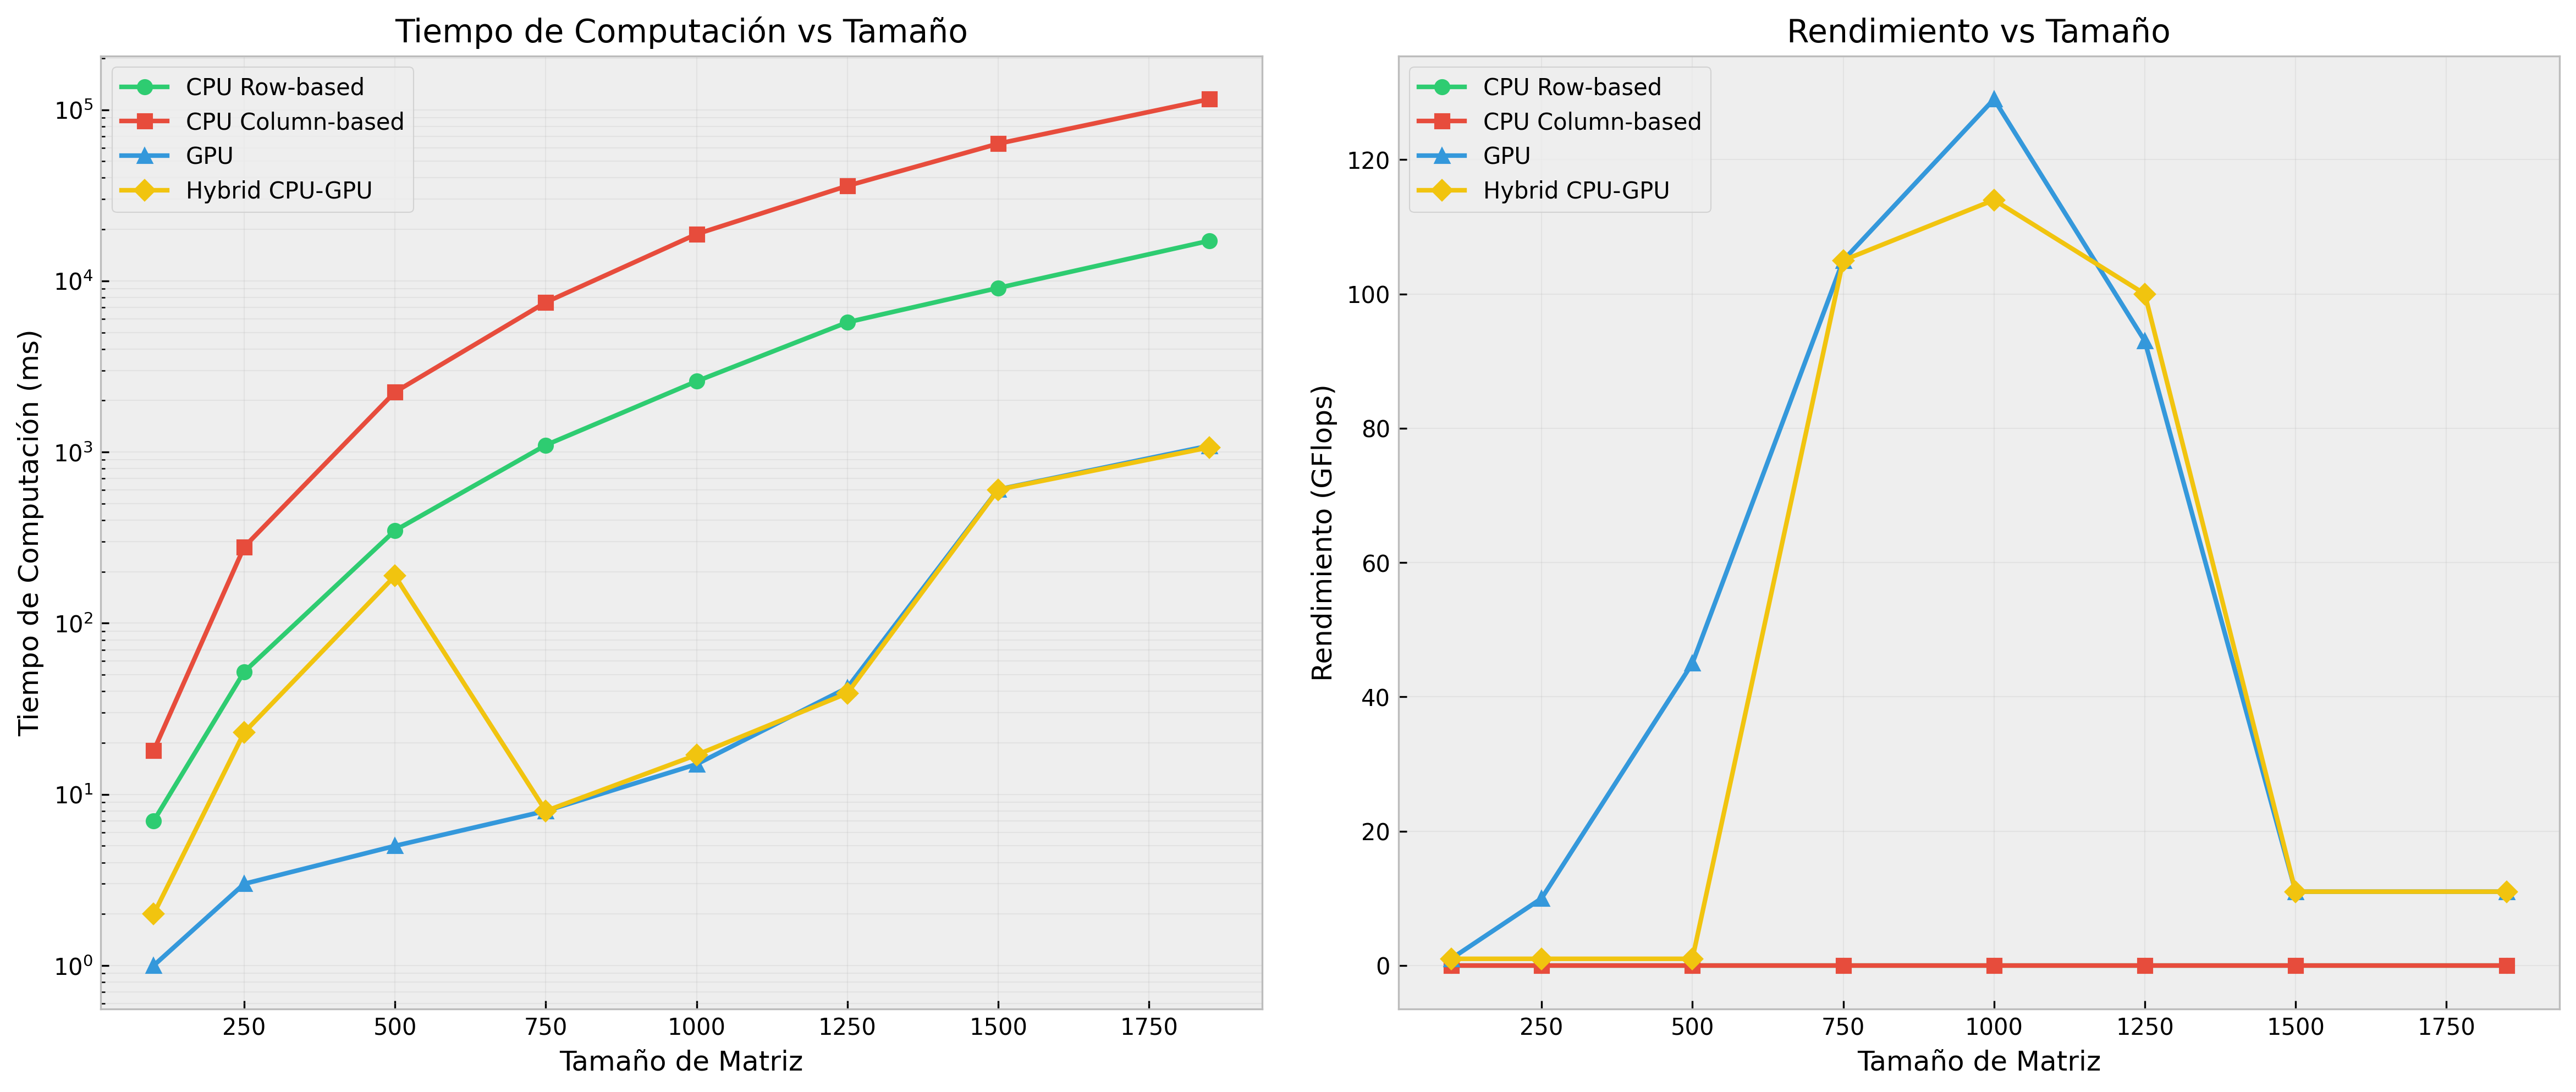
\includegraphics[width=0.8\textwidth]{./grafica.png}
    \caption{Comparación de rendimiento entre multiplicación por filas vs columnas vs GPU}
\end{figure}

\subsection{Análisis de Rendimiento}
\subsubsection{Implementaciones CPU}
\begin{itemize}
    \item \textbf{Localidad espacial:} El acceso por filas aprovecha mejor la estructura de memoria cache
    \item \textbf{Patrones de acceso:} El acceso por columnas genera más fallos de caché
    \item \textbf{Paralelización:} Ambas implementaciones utilizan \texttt{Parallel.For} para distribuir la carga
\end{itemize}

\subsubsection{Implementación GPU}
\begin{itemize}
    \item \textbf{Paralelismo masivo:} Aprovecha miles de núcleos de procesamiento simultáneo
    \item \textbf{Overhead de transferencia:} El tiempo incluye la transferencia de datos entre CPU y GPU
    \item \textbf{Eficiencia escalar:} Mayor beneficio en matrices grandes donde el paralelismo compensa el overhead
\end{itemize}

\section{Conclusiones}
La implementación GPU demuestra ventajas significativas en matrices de gran tamaño, donde el paralelismo masivo compensa el overhead de transferencia de datos. Las implementaciones CPU optimizadas mantienen buena eficiencia para tamaños pequeños y medianos, especialmente la versión por filas debido a su mejor utilización de la caché.

\section{Trabajo Futuro}
\begin{itemize}
    \item Optimización de patrones de acceso a memoria en GPU
    \item Implementación de algoritmos de multiplicación por bloques en GPU
    \item Análisis con matrices dispersas
    \item Estudio del impacto de diferentes tamaños de grupo de trabajo en OpenCL
    \item Comparación con otras APIs de GPU como DirectCompute
\end{itemize}

\end{document}